\chapter{Aplicação da ontologia no software}
  
  Atualmente, o ``Pé na estrada'' disponibiliza informações apenas sobre os locais dos
  acidentes, e a quantidade de acidentes em cada rodovia. Esse tipo de informação seria mais
  relevante se acompanhassem informações acerca dos tipos de acidentes, danos causados a
  rodovia, tipo de veículo, envolvidos, entre outros dados que fossem relevantes para análise
  estatística e para representação gráfica.

  Dessa forma, com o modelo de dados estruturado semanticamente, esses dados seriam
  encontrados e relacionados facilmente, possibilitando ao software disponibilizar essas
  informações ao usuário, até mesmo de forma mais visual.

  Atualmente, o software não possui nenhuma camada semântica presente, possuindo
  apenas a camada visual do HTML, sendo necessária toda a estruturação das três principais
  camadas semânticas: o XML, o RDFS e a OWL, sendo esta última necessária para o uso da
  ontologia que será criada para representar os acidentes de trânsito.

  Para fazer a comunicação da aplicação com a ontologia definida é necessário substituir a comunicação da \textit{Model} que ao invés
  de estabelecer relação com a \textit{Active Record} deve estabelecer relação com dados em RDF.

  Existe um \textit{framework} chamado \textit{Active RDF} \footnotemark[1] que substitui a \textit{Active Record} e estabelece um relacionamento
  do sistema com os dados contidos na ontologia. Infelizmente, esse \textit{framework} não é mais mantido, o que compromete a sua utilização no projeto.
  \footnotetext[1]{http://www.activerdf.org/}
  
  Para ainda assim conseguir trazer uma camada semântica para o software, foi utilizado um banco de dados orientado a grafos, o Neo4J, para
  substituir a ontologia, uma vez que a ideia de ontologia se baseia no conceito de grafo, sendo perfeitamente possível representar
  uma ontologia como um grafo.
  
   \section{Modelagem das entidades}
    
    O principal relacionamento existente no ``Pé na estrada'' é dado pelas entidades Acidente e Rodovia, onde acidentes
    acontecem em uma Rodovia. Atualmente é feito um mapeamento relacional de ``um para muitos'' entre Rodovia e Acidente.
    
    Para utilizar o Neo4j no Rails existe uma biblioteca chamada Neo4j.rb \footnotemark que abstrai o acesso à instância do Neo4j e
    oferece classes para facilitar a modelagem em Ruby.
    O relacionamento foi mapeado para o Neo4J utilizando recursos do Neo4J.rb e as entidades na aplicação ficaram assim:
    \footnotetext{https://github.com/neo4jrb/neo4j}
    
    
    \lstset{language=Ruby}
    \begin{lstlisting}[frame=single]
    
      class Accident
	include Neo4j::ActiveNode

	property :latitude
	property :longitude
	property :uf
	property :km

	has_one :out, :highway,
		type: :highway,
		model_class: :Highway
      end
      
      class Highway
	include Neo4j::ActiveNode

	property :br
	property :mileage

	has_many :in, :accidents,
		 origin: :highway,
		 model_class: :Accident
      end

    \end{lstlisting}
    
    Embora essa modelagem inicial seja bastante simples (contando apenas com duas entidades),
    com essa nova estrutura de classes na camada \textit{Model}, já temos uma melhor representação
    dos dados e uma interface de consulta mais poderosa.
    
    \vfill
    \pagebreak
    
    \section{Testes da nova modelagem}
    
      Para testar a nova estrutura orientada a grafos das \textit{models}, o banco de dados foi carregado
      com parte dos dados dos acidentes do primeiro semestre de 2014 fornecidos pela PRF.
      
      Foram carregados aproximadamente 13300 registros de acidentes e foi possível realizar as mesmas atividades
      realizadas anteriormente com o modelo relacional. Em questões de performance o banco de dados orientado a 
      grafos perde um pouco para o banco de dados relacional, mas compensa pelo poder de semântica oferecido.
      
      A Figura \ref{fig:db_general_view} ilustra uma parte do banco de dados, mostrando as rodovias, acidentes 
      e seus respectivos relacionamentos cadastrados no Neo4j. Cada ``bolinha'' pode ser tanto uma rodovia quanto
      um acidente. Caso seja uma acidente, terá um relacionamento o ligando a outro registro, pois não existem acidentes
      que não aconteceram em uma rodovia. Registros isolados são rodovias que não possuem acidentes registrados.
      
      \begin{figure}[!h]
	\centering
	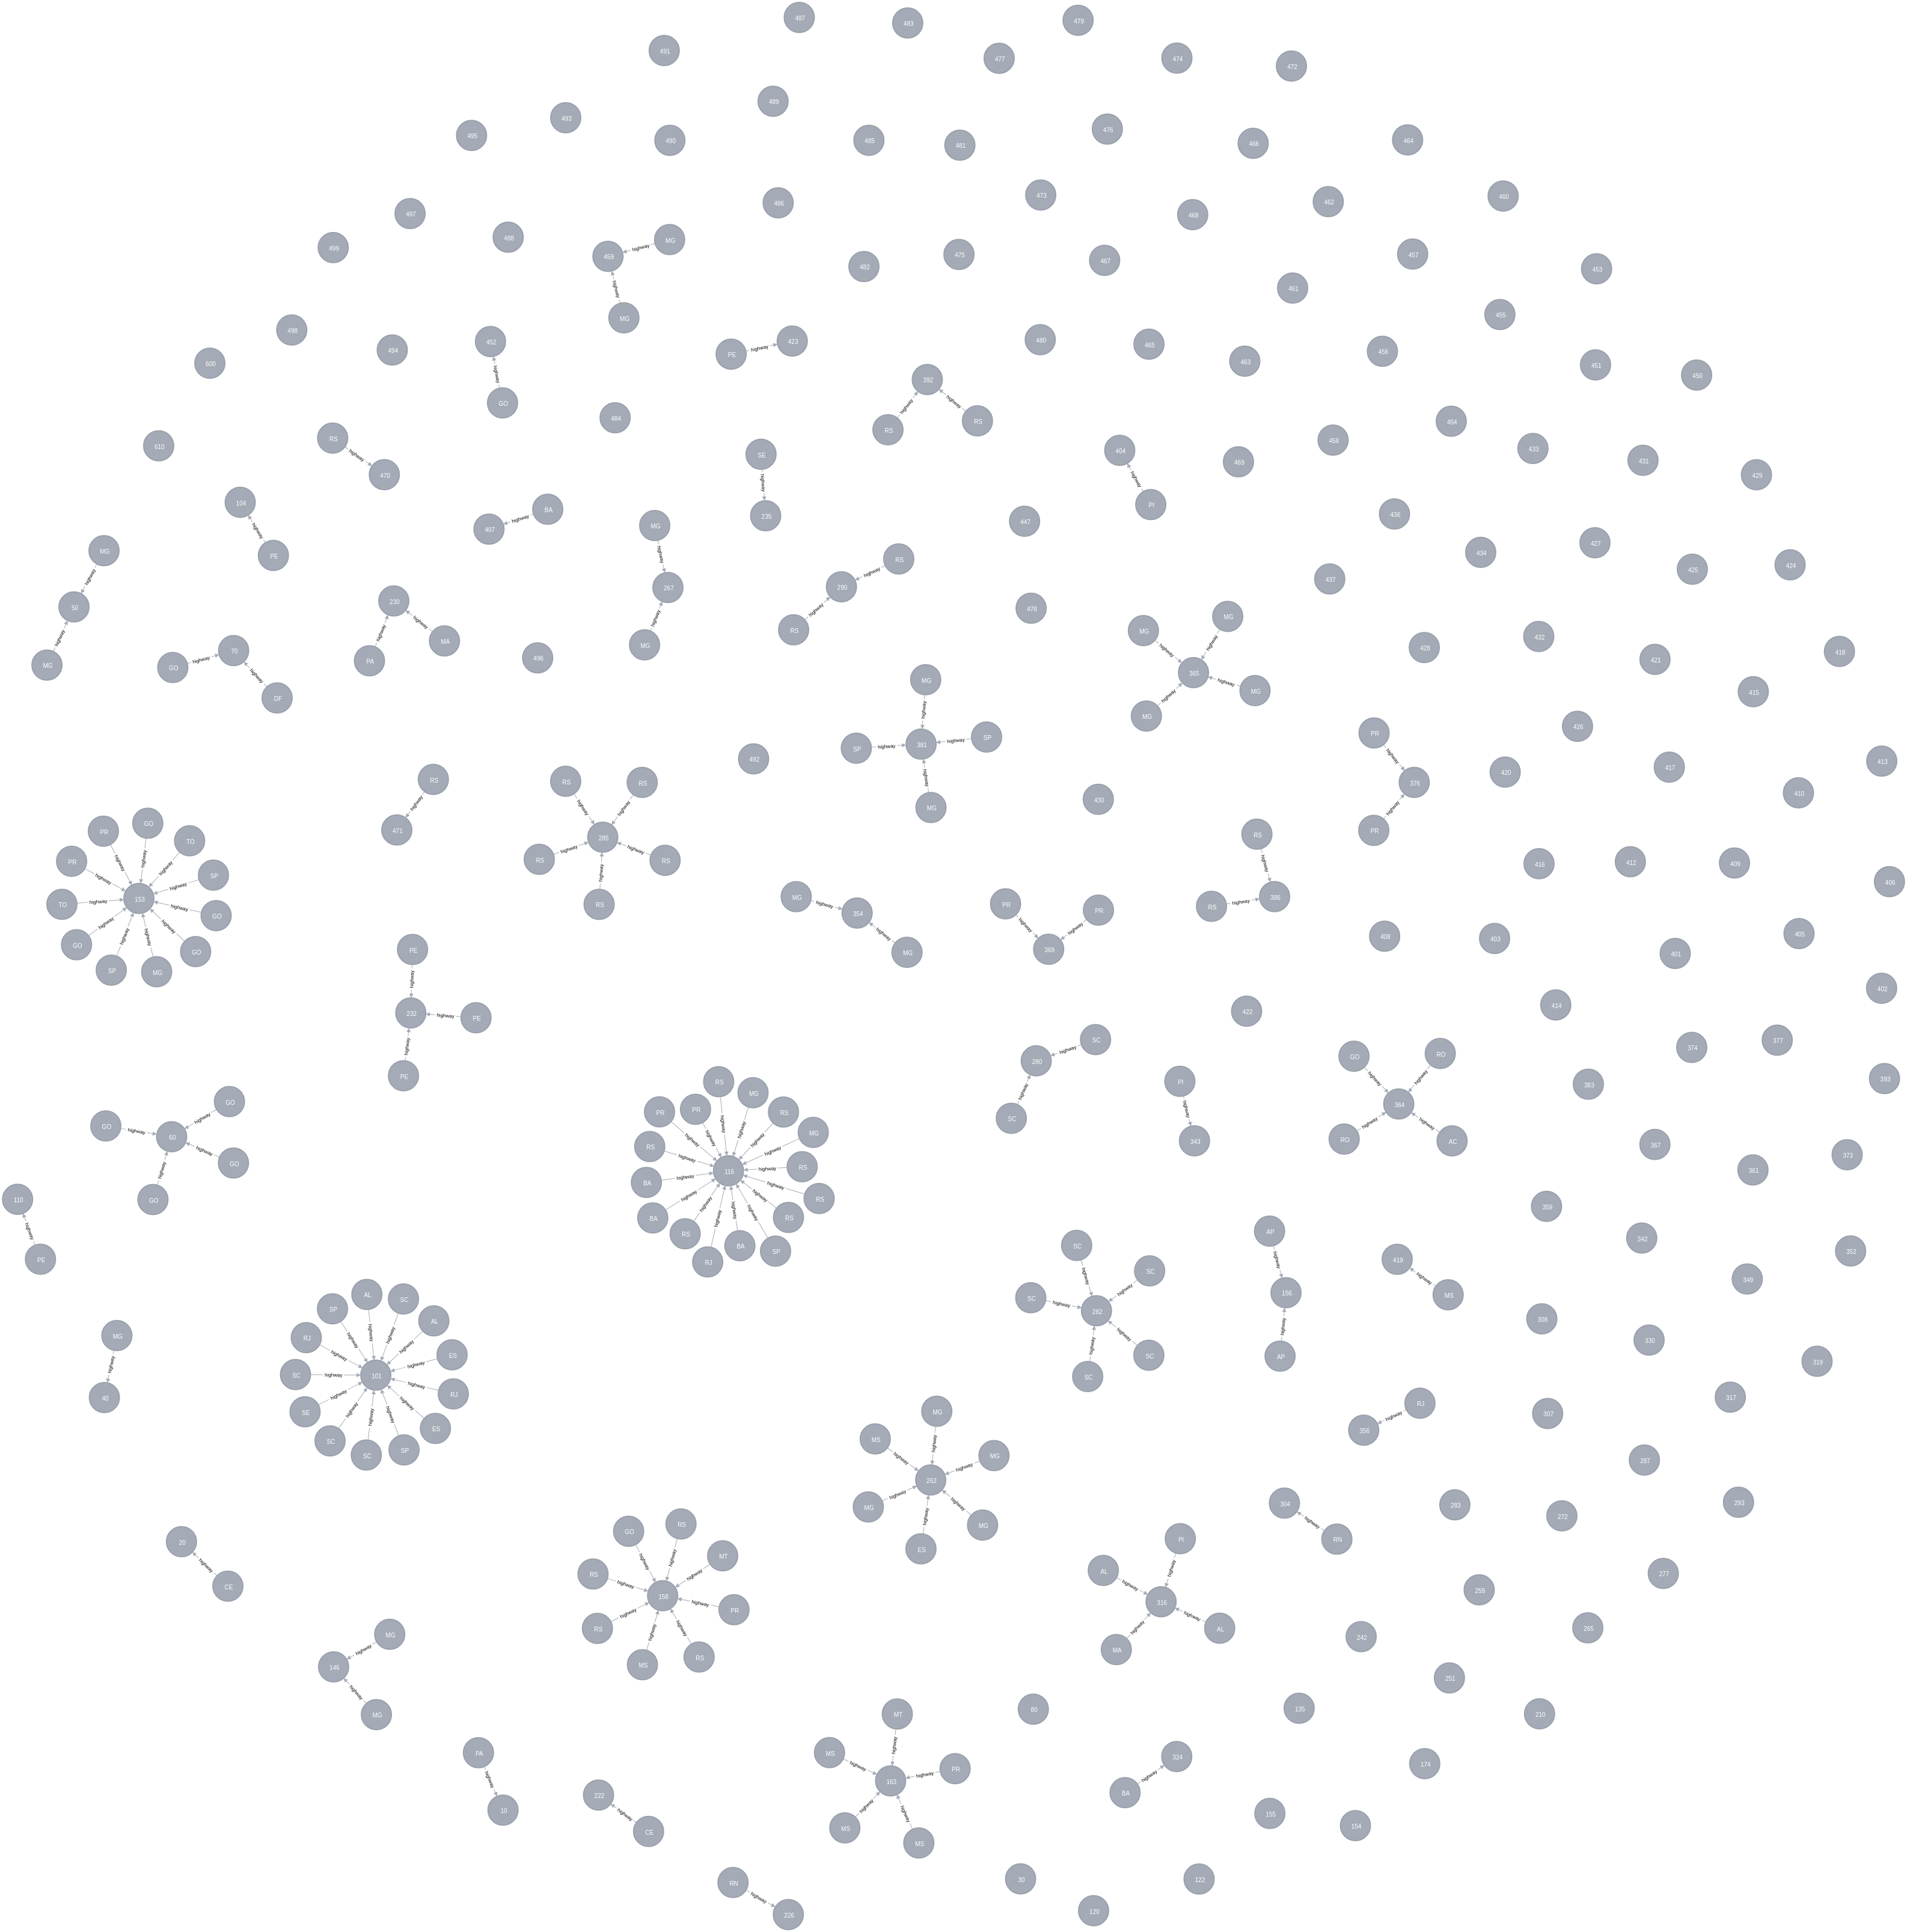
\includegraphics[scale = 0.1]{figuras/graph.png}
	\caption[Visão geral do banco de dados]{Visão geral do banco de dados. \textit{Imagem gerada pelo Neo4j.}}
	\label{fig:db_general_view}
      \end{figure}
      
      A Figura \ref{fig:db_example} apresenta um exemplo de três rodovias registradas no banco de dados, BR-285, BR-354 e BR-430.
      Como foi mencionado, cada ``bolinha'' representa um registro e cada ``seta'' representa uma relação entre os registros.
      No caso da \ref{fig:db_example} a relação ``\textit{highway}'' representa que aquela rodovia é o local do acidente.
      Neste exemplo é possível ver que ocorreram cinco acidentes na rodovia BR-285 no estado do Rio Grande de Sul, dois acidentes
      na BR-354 no estado de Minas Gerais e não ocorreram acidentes na rodovia BR-430.
      
      
      \begin{figure}[!h]
	\centering
	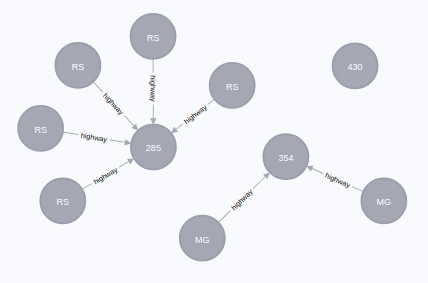
\includegraphics[scale = 0.7]{figuras/db_example.png}
	\caption[Exemplo de registros no banco de dados]{Exemplo de registros no banco de dados. \textit{Imagem gerada pelo Neo4j.}}
	\label{fig:db_example}
      \end{figure}
      
      \subsection*{Comparação com o banco de dados relacional}
      
	Considerando o cenário de recuperar a quantidade de acidentes
	ocorridos na rodovia BR-116 pelo nome da rodovia, a respectiva
	consulta em SQL ficaria assim:
      
	\lstset{language=SQL}
	\begin{lstlisting}[frame=single, caption=Consulta em SQL]
	  SELECT COUNT(*) FROM accidents
	  INNER JOIN highways 
	    ON highways.id = accidents.highway_id
	  WHERE highways."br" = '116'
	\end{lstlisting}
	
	Já em CYPHER (linguagem de consulta do Neo4j) ficaria assim:
	
	\lstset{language=SQL}
	\begin{lstlisting}[frame=single]
	  MATCH (node:`Accident`) 
	  MATCH (node)-[rel1:`highway`]->(result_highway:`Highway`)
	  WHERE (result_highway.br = {result_highway_br})
	  RETURN count(result_highway) 
	    AS result_highway | {:result_highway_br=>"116"}
	\end{lstlisting}

	Em relação a performance, para 13300 registros, o banco de dados relacional
	consegue responder a esta consulta em uma média de 3ms,
	enquanto o banco de dados orientado a grafos responde em 17ms.